\textbf{Цель работы:} Получение навыков разработки алгоритмов решения смешанной краевой задачи при реализации моделей, построенных на квазиинейном уравнении параболического типа.

\section{ИСХОДНЫЕ ДАННЫЕ}

\subsection{Задана математическая модель}

Уравнение для функции $T(x, t)$ (формула \ref{eq:main_t}).

\begin{equation}\label{eq:main_t}
    c(T) \frac{\partial T}{\partial t} = \frac{\partial}{\partial x} \bigg( k(T) \frac{\partial T}{\partial x} \bigg) - \frac{2}{R} \alpha(x) T + \frac{2T_0}{R} \alpha(x)
\end{equation}

Краевые условия

\begin{equation*}
    \begin{cases}
        t = 0, T(x, 0) = T_0 \\
        x = 0, -k \big( T(0) \big) \frac{\partial T}{\partial x} = F_0 \\
        x = l, -k \big( T(l) \big) \frac{\partial T}{\partial x} = \alpha_N \big( T(l) - T_0 \big) \\
    \end{cases}
\end{equation*}

Функция $\alpha (x)$

\begin{equation*}
    \alpha(x) = \frac{c}{x-d}
\end{equation*}

, где

\begin{equation*}
    c = -\alpha_0 d = \frac{\alpha_0 \alpha_N l}{\alpha_0 - \alpha_N}
\end{equation*}

\begin{equation*}
    d = \frac{\alpha_N l}{\alpha_N - \alpha_0}
\end{equation*}

\subsection{Разностная схема}

Систему квазилинейных растностных уравнений видно на формуле \ref{eq:system_diff}.

\begin{equation}\label{eq:system_diff}
    \begin{cases}
        \LittleCap{K}_0 \LittleCap{y}_0 + \LittleCap{M}_0 \LittleCap{y}_1 = \LittleCap{P}_0 \\
        \LittleCap{A}_n \LittleCap{y}_{n-1} - \LittleCap{B}_n \LittleCap{y}_n + \LittleCap{D}_n \LittleCap{y}_{n+1} = - \LittleCap{F}_n,\ \ 1 \le n \le N - 1 \\
        \LittleCap{K}_N \LittleCap{y}_N + \LittleCap{M}_{N-1} \LittleCap{y}_{N-1} = \LittleCap{P}_N \\
    \end{cases}
\end{equation}

\begin{equation*}
    \begin{matrix*}[l]
        \LittleCap{A}_n = \LittleCap{\chi}_{n-\frac{1}{2}} \frac{\tau}{h} \\
        \LittleCap{B}_n = \LittleCap{A}_n + \LittleCap{D}_n + \LittleCap{c}_n h + p_n h \tau \\
        \LittleCap{D}_n = \LittleCap{\chi}_{n + \frac{1}{2}} \frac{\tau}{h} \\
        \LittleCap{F}_n = f_n h \tau + \LittleCap{c}_n y_n h \\
    \end{matrix*}
\end{equation*}

\subsection{Краевые условия}

Обозначим:

\begin{equation*}
    \begin{matrix*}[l]
        F = - k(T) \frac{\partial T}{\partial x} \\
        p(x) = \frac{2}{R} \alpha(x) \\
        f(x) = \frac{2T_0}{R} \alpha(x) \\
    \end{matrix*}
\end{equation*}

Разностный аналог краевого условия при $x=0$

\begin{multline}\label{eq:diff_x0}
    \bigg( \frac{h}{8} \LittleCap{c}_\frac{1}{2} +\ \frac{h}{4} \LittleCap{c}_0 + \LittleCap{\chi}_\frac{1}{2} \frac{\tau}{h} + \frac{\tau h}{8} p_\frac{1}{2} + \frac{\tau h}{4} p_0 \bigg) \LittleCap{y}_0 + \bigg( \frac{h}{8} \LittleCap{c}_\frac{1}{2} - \LittleCap{\chi}_\frac{1}{2} \frac{\tau}{h} + \frac{\tau h}{8} p_\frac{1}{2} \bigg) \LittleCap{y}_1 = \\
    = \frac{h}{8} \LittleCap{c}_\frac{1}{2} \big( y_0 + y_1 \big) + \frac{h}{4} \LittleCap{c}_0 y_0 + \LittleCap{F}\tau + \frac{\tau h}{4} \big(\LittleCap{f}_\frac{1}{2} + \LittleCap{f}_0 \big)
\end{multline}

Получим разностный аналог краевого условия $x=l$. Проинтегрируем уравнение \ref{eq:main_t} на отрезке $[x_{N-\frac{1}{2}}, x_N]$ и на временном интервале $[t_m, t_{m+1}]$.

\begin{multline*}
    \int_{x_{N-\frac{1}{2}}}^{x_N} dx \int_{t_m}^{t_{m+1}} c(T) \frac{\partial T}{\partial t} dt = - \int_{t_m}^{t_{m+1}} dt \int_{x_{N-\frac{1}{2}}}^{x_N} \frac{\partial F}{\partial x} dx - \\
    - \int_{x_{N-\frac{1}{2}}}^{x_N} dx \int_{t_m}^{t_{m+1}} p(x) T dt + \int_{x_{N-\frac{1}{2}}}^{x_N} dx \int_{t_m}^{t_{m+1}} f(T) dt
\end{multline*}

\begin{equation*}
    \int_{x_{N-\frac{1}{2}}}^{x_N} \LittleCap{c} (\LittleCap{T} -\ T) dx = - \int_{t_m}^{t_{m+1}} \big( F_N - F_{N - \frac{1}{2}} \big) dt - \int_{x_{N-\frac{1}{2}}}^{x_N} p \LittleCap{T} \tau dx + \int_{x_{N - \frac{1}{2}}}^{x_N} \LittleCap{f} \tau dx
\end{equation*}

\begin{multline*}
    \frac{h}{4} \big[ \LittleCap{c}_N \big( \LittleCap{y}_N -\ y_N \big) + \LittleCap{c}_{N-\frac{1}{2}} \big( \LittleCap{y}_{N-\frac{1}{2}} -\ y_{N-\frac{1}{2}} \big) \big] = - \big( \LittleCap{F}_N - \LittleCap{F}_{N-\frac{1}{2}} \big) \tau - \\
    - \big( p_N \LittleCap{y}_N +\ p_{N-\frac{1}{2}} \LittleCap{y}_{N-\frac{1}{2}} \big) \tau \frac{h}{4} + \big( \LittleCap{f}_N + \LittleCap{f}_{N-\frac{1}{2}} \big) \tau \frac{h}{4}
\end{multline*}

Подставим \ref{eq:cap_y_1_2}, \ref{eq:y_1_2}, \ref{eq:F_N} и \ref{eq:F_N-1_2}.

\begin{equation}\label{eq:cap_y_1_2}
    \LittleCap{y}_{N-\frac{1}{2}} = \frac{\LittleCap{y}_{N-1} + \LittleCap{y}_N}{2}
\end{equation}

\begin{equation}\label{eq:y_1_2}
    y_{N-\frac{1}{2}} = \frac{y_{N-1} + y_N}{2}
\end{equation}

\begin{equation}\label{eq:F_N}
    \LittleCap{F}_N = \alpha_N \big( \LittleCap{y}_N - T_0 \big)
\end{equation}

\begin{equation}\label{eq:F_N-1_2}
    \LittleCap{F}_{N-\frac{1}{2}} = \LittleCap{\chi}_{N-\frac{1}{2}} \frac{\LittleCap{y}_{N-1} - \LittleCap{y}_N}{h}
\end{equation}

Получим

\begin{multline}\label{eq:diff_xl}
    \LittleCap{y}_N \bigg( \frac{h}{4} \LittleCap{c}_N +\ \frac{h}{8} \LittleCap{c}_{N-\frac{1}{2}} + \alpha_N \tau + \LittleCap{\chi}_{N-\frac{1}{2}} \frac{\tau}{h} + p_N \frac{\tau h}{4} + p_{N-\frac{1}{2}} \frac{\tau h}{8} \bigg) + \\
    + \LittleCap{y}_{N-1} \bigg( \frac{h}{8} \LittleCap{c}_{N-\frac{1}{2}} - \LittleCap{\chi}_{N-\frac{1}{2}} \frac{\tau}{h} + p_{N-\frac{1}{2}} \frac{\tau h}{8} \bigg) = \\
    = \frac{h}{4} \LittleCap{c}_N y_N + \frac{h}{8} \LittleCap{c}_{N-\frac{1}{2}} y_{N-1} + \frac{h}{8} \LittleCap{c}_{N-\frac{1}{2}} y_N + T_0 \alpha_N \tau + \big( \LittleCap{f}_N + \LittleCap{f}_{N-\frac{1}{2}} \big) \frac{\tau h}{4}
\end{multline}

С помощью формул \ref{eq:system_diff} и \ref{eq:diff_x0} получим коэффициенты $\LittleCap{K}_0, \LittleCap{M}_0, \LittleCap{P}_0$, а с помощью \ref{eq:system_diff} и \ref{eq:diff_xl} -- $\LittleCap{K}_N, \LittleCap{M}_{N-1}, \LittleCap{P}_N$.

\subsection{Метод простых итераций}

Для решения системы \ref{eq:system_diff} используется метод простых итераций. Обозначим текущую итерацию за $s$, тогда предыдущая -- $s - 1$. С данными обозначениями итерационный процесс организуется следующим образом

\begin{equation*}
    A_n^{s-1} y_{n+1}^s - B_{n}^{s-1} y_n^s + D_n^{s-1} y_{n-1}^s = -F_n^{s-1}
\end{equation*}

Решение данной схемы осуществляется методом прогонки. Итерации прекращаются при условии

\begin{equation*}
    \max \bigg| \frac{y_n^s - y_n^{s-1}}{y_n^s} \bigg| \le \varepsilon, n = \overline{0;N}
\end{equation*}

\subsection{Значения параметров для отладки}

\begin{equation*}
    \begin{matrix*}[l]
        k(T) = a_1(b_1 + c_1 T^{m_1}), \frac{\text{Вт}}{\text{см К}}, \\
        c(T) = a_2 + b_2 T^{m_2} - \frac{c_2}{T^2}, \frac{\text{Дж}}{\text{см}^3 \text{К}}, \\
        a_1 = 0.0134,\ b_1 = 1,\ c_1 = 4.35 \cdot 10^{-4},\ m_1=1, \\
        a_2 = 2.049,\ b_2 = 0.563 \cdot 10^{-3},\ c_2 = 0.528 \cdot 10^5,\ m_2 = 1 \\
        \alpha(x) = \frac{c}{x-d}, \\
        \alpha_0 = 0.05\ \frac{\text{Вт}}{\text{см}^2 \text{К}}, \\
        \alpha_N = 0.01\ \frac{\text{Вт}}{\text{см}^2 \text{К}}, \\
        l = 10\ \text{см}, \\
        T_0 = 300\ \text{К}, \\
        R = 0.5\ \text{см} \\
        F(t) = 50 \frac{\text{Вт}}{\text{см}^2}.
    \end{matrix*}
\end{equation*}

\section{ЛИСТИНГИ}

\begin{lstlisting}[caption=Теплоемкость стержня]
double Mathematics::c(const double T)
{
    return _a2 + _b2 * std::pow(T, _m2) - _c2 / (T * T);
}
\end{lstlisting}

\begin{lstlisting}[caption=Коэффициент теплопроводности стержня]
double Mathematics::k(const double T)
{
    return _a1 * (_b1 + _c1 * std::pow(T, _m1));
}
\end{lstlisting}

\begin{lstlisting}[caption=Коэффициент теплоотдачи при обдуве]
double Mathematics::alpha(const double x)
{
    double d = (_alphaN * _l) / (_alphaN - _alpha0);
    double c = -_alpha0 * d;
    return c / (x - d);
}
\end{lstlisting}

\begin{lstlisting}[caption=Замены p и f]
double Mathematics::p(const double x)
{
    return (2.0 / _R) * alpha(x);
}

double Mathematics::f(const double x)
{
    return (2.0 * _T0 / _R) * alpha(x);
}
\end{lstlisting}

\begin{lstlisting}[caption=Метод средних для всех функций]
double Mathematics::chi1_2(const double T, const double tau)
{
    return (k(T) + k(T + tau)) / 2.0;
}

double Mathematics::c1_2(const double T, const double tau)
{
    return (c(T) + c(T + tau)) / 2.0;
}

double Mathematics::p1_2(const double x, const double h)
{
    return (p(x) + p(x + h)) / 2.0;
}

double Mathematics::f1_2(const double x, const double h)
{
    return (f(x) + f(x + h)) / 2.0;
}
\end{lstlisting}

\begin{lstlisting}[caption=Параметры разностной схемы]
double Mathematics::A(const double T)
{
    return chi1_2(T, -_tau) * _tau / _h;
}

double Mathematics::B(const double T, const double x)
{
    return A(T) + D(T) + c(T) * _h + p(x) * _h * _tau;
}

double Mathematics::D(const double T)
{
    return chi1_2(T, _tau) * _tau / _h;
}

double Mathematics::F(const double T, const double x)
{
    return f(x) * _h * _tau + c(T) * T * _h;
}
\end{lstlisting}

\begin{lstlisting}[caption=Метод прогонки]
QVector<double> Mathematics::runTrought(const QVector<double> &prev)
{
    const double K0 = _h / 8.0 * c1_2(prev[0], _tau) +
        _h / 4.0 * c(prev[0]) + chi1_2(prev[0], _tau) *
        _tau / _h + _tau * _h / 8.0 * p1_2(0, _h) +
        _tau * _h / 4.0 * p(0);
    const double M0 = _h / 8.0 * c1_2(prev[0], _tau) -
        chi1_2(prev[0], _tau) * _tau / _h +
        _tau * _h / 8.0 * p1_2(0, _h);
    const double P0 = _h / 8.0 * c1_2(prev[0], _tau) * (prev[0] + prev[1]) +
        _h / 4.0 * c(prev[0]) * prev[0] +
        _Ft * _tau +
        _tau * _h / 4.0 * (f1_2(0, _h) + f(0));

    const double KN = _h / 4.0 * c(prev.last()) +
        _h / 8.0 * c1_2(prev.last(), -_tau) +
        _alphaN * _tau +
        chi1_2(prev.last(), -_tau) * _tau / _h +
        p(_l) * _tau * _h / 4.0 +
        p1_2(_l, -_h) * _tau * _h / 8.0;
    const double MN = _h / 8.0 * c1_2(prev.last(), -_tau) -
        chi1_2(prev.last(), -_tau) * _tau / _h +
        p1_2(_l, -_h) * _tau * _h / 8.0;
    const double PN = _h / 4.0 * c(prev.last()) * prev.last() +
        _h / 8.0 * c1_2(prev.last(), -_tau) * prev[prev.count() - 2] +
        _h / 8.0 * c1_2(prev.last(), -_tau) * prev.last() +
        _T0 * _alphaN * _tau +
        (f(_l) + f1_2(_l, -_h)) * _tau * _h / 4.0;

    QVector<double> eps;
    eps.append(-M0 / K0);

    QVector<double> eta;
    eta.append(P0 / K0);

    int n = 1;
    for (double x = _h; x + _h < _l; x += _h, n += 1) {
        double epsN = eps.last();
        double etaN = eta.last();
        eps.append(D(prev[n]) / (B(prev[n], x) - A(prev[n]) * epsN));
        eta.append((F(prev[n], x) + A(prev[n]) * etaN) /
            (B(prev[n], x) - A(prev[n]) * epsN));
    }

    QVector<double> t(eps.count());
    t[t.count() - 1] = (PN - MN * eta.last()) / (KN + MN * eps.last());

    for (int i = t.count() - 2; i >= 0; --i) {
        t[i] = eps[i + 1] * t[i + 1] + eta[i + 1];
    }

    return t;
}
\end{lstlisting}

\begin{lstlisting}[caption=Метод простых итераций]
void Mathematics::iterations()
{
    if (!_secondRun) {
        QVector<double> tZero;
        int n = int(_l / _h) + 1;
        for (int i = 0; i < n; ++i) {
            if (_anotherStart) {
                tZero.append(1000);
            } else {
                tZero.append(_T0);
            }
        }

        temp.append(tZero);
    }

    do {
        QVector<double> prev;
        QVector<double> curr = temp.last();

        do {
            prev = curr;
            curr = runTrought(prev);
        } while (!endRunTrought(prev, curr));

        temp.append(curr);
    } while (!endIterations());
}
\end{lstlisting}

\begin{lstlisting}[caption=Условие завершения прогонки]
bool Mathematics::endRunTrought(
    const QVector<double> &prev,
    const QVector<double> &current
)
{
    double max = std::fabs((current[0] - prev[0]) / current[0]);

    for (int i = 1; i < std::min(current.count(), prev.count()); ++i) {
        double e = std::fabs((current[i] - prev[i]) / current[i]);

        if (e > max)
            max = e;
    }

    return max < _eps;
}
\end{lstlisting}

\begin{lstlisting}[caption=Условие завершения метода простых итераций]
bool Mathematics::endIterations()
{
    int last = temp.count() - 1;
    for (int i = 0; i < temp[last].count(); ++i) {
        if (std::fabs(
                (temp[last][i] - temp[last - 1][i]) / temp[last][i]
            ) > _eps)
            return false;
    }

    return true;
}
\end{lstlisting}

\begin{lstlisting}[caption=Запуск вычислений]
Mathematics::Mathematics(
    const double alpha0, const double alphaN, const double l,
    const double T0, const double R, const double Ft,
    const bool again, const bool another
) : _alpha0(alpha0), _alphaN(alphaN), _l(l),
    _T0(T0), _R(R), _Ft(Ft),
    _again(again), _anotherStart(another)
{
    if (_anotherStart) {
        _Ft = 0;
    }

    iterations();

    if (_again) {
        _Ft = 0;
        _secondRun = true;
        iterations();
    }
}
\end{lstlisting}

\section{РЕЗУЛЬТАТЫ РАБОТЫ}

На рисунке \ref{img:defaultTm} представлен график зависимости температуры от координаты стержня при фиксированных значениях времени $t$. На этом графике последняя кривая, оранжевая, соответствет установившемуся режиму, когда поле перестанет меняться с точностью $10^{-4}$.

\begin{figure}[H]
    \centering
    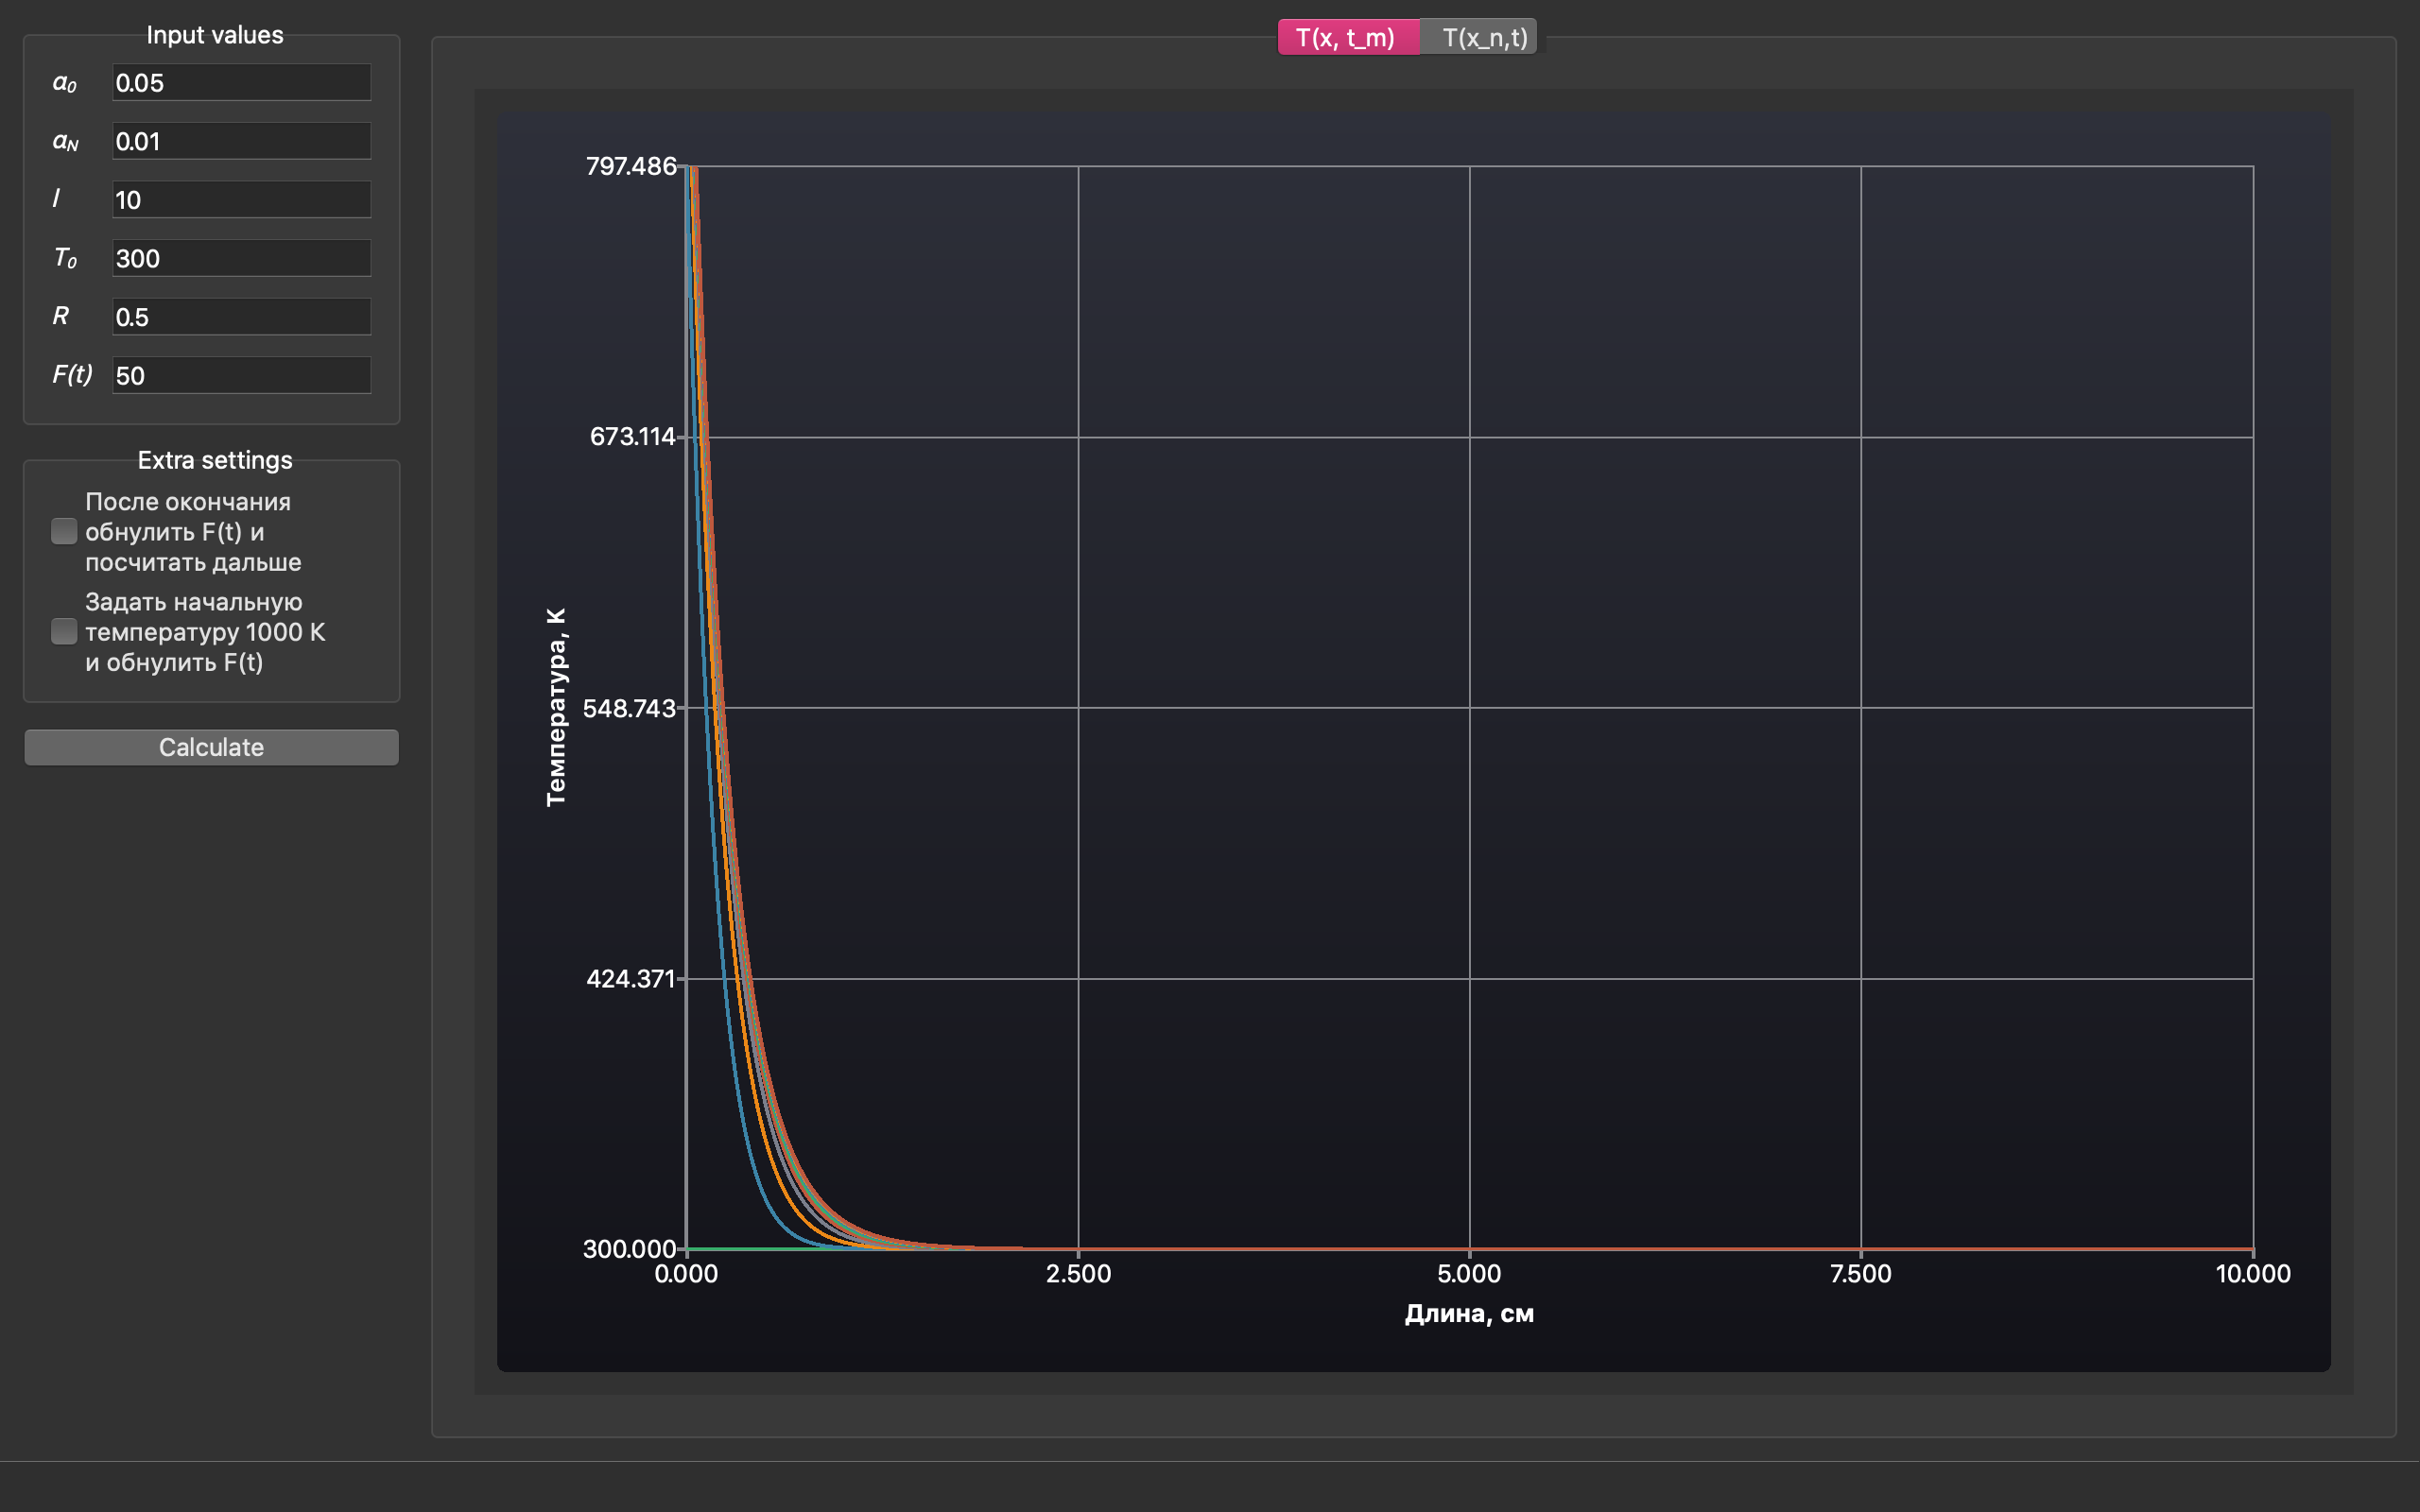
\includegraphics[scale=0.35]{img/defaultTm.png}
    \caption{Зависимость температуры от координаты стержня}
    \label{img:defaultTm}
\end{figure}

На рисунке \ref{img:defaultXn} представлен график зависимости температуры от времени при нескольких фиксированных значениях координаты $x$.

\begin{figure}[H]
    \centering
    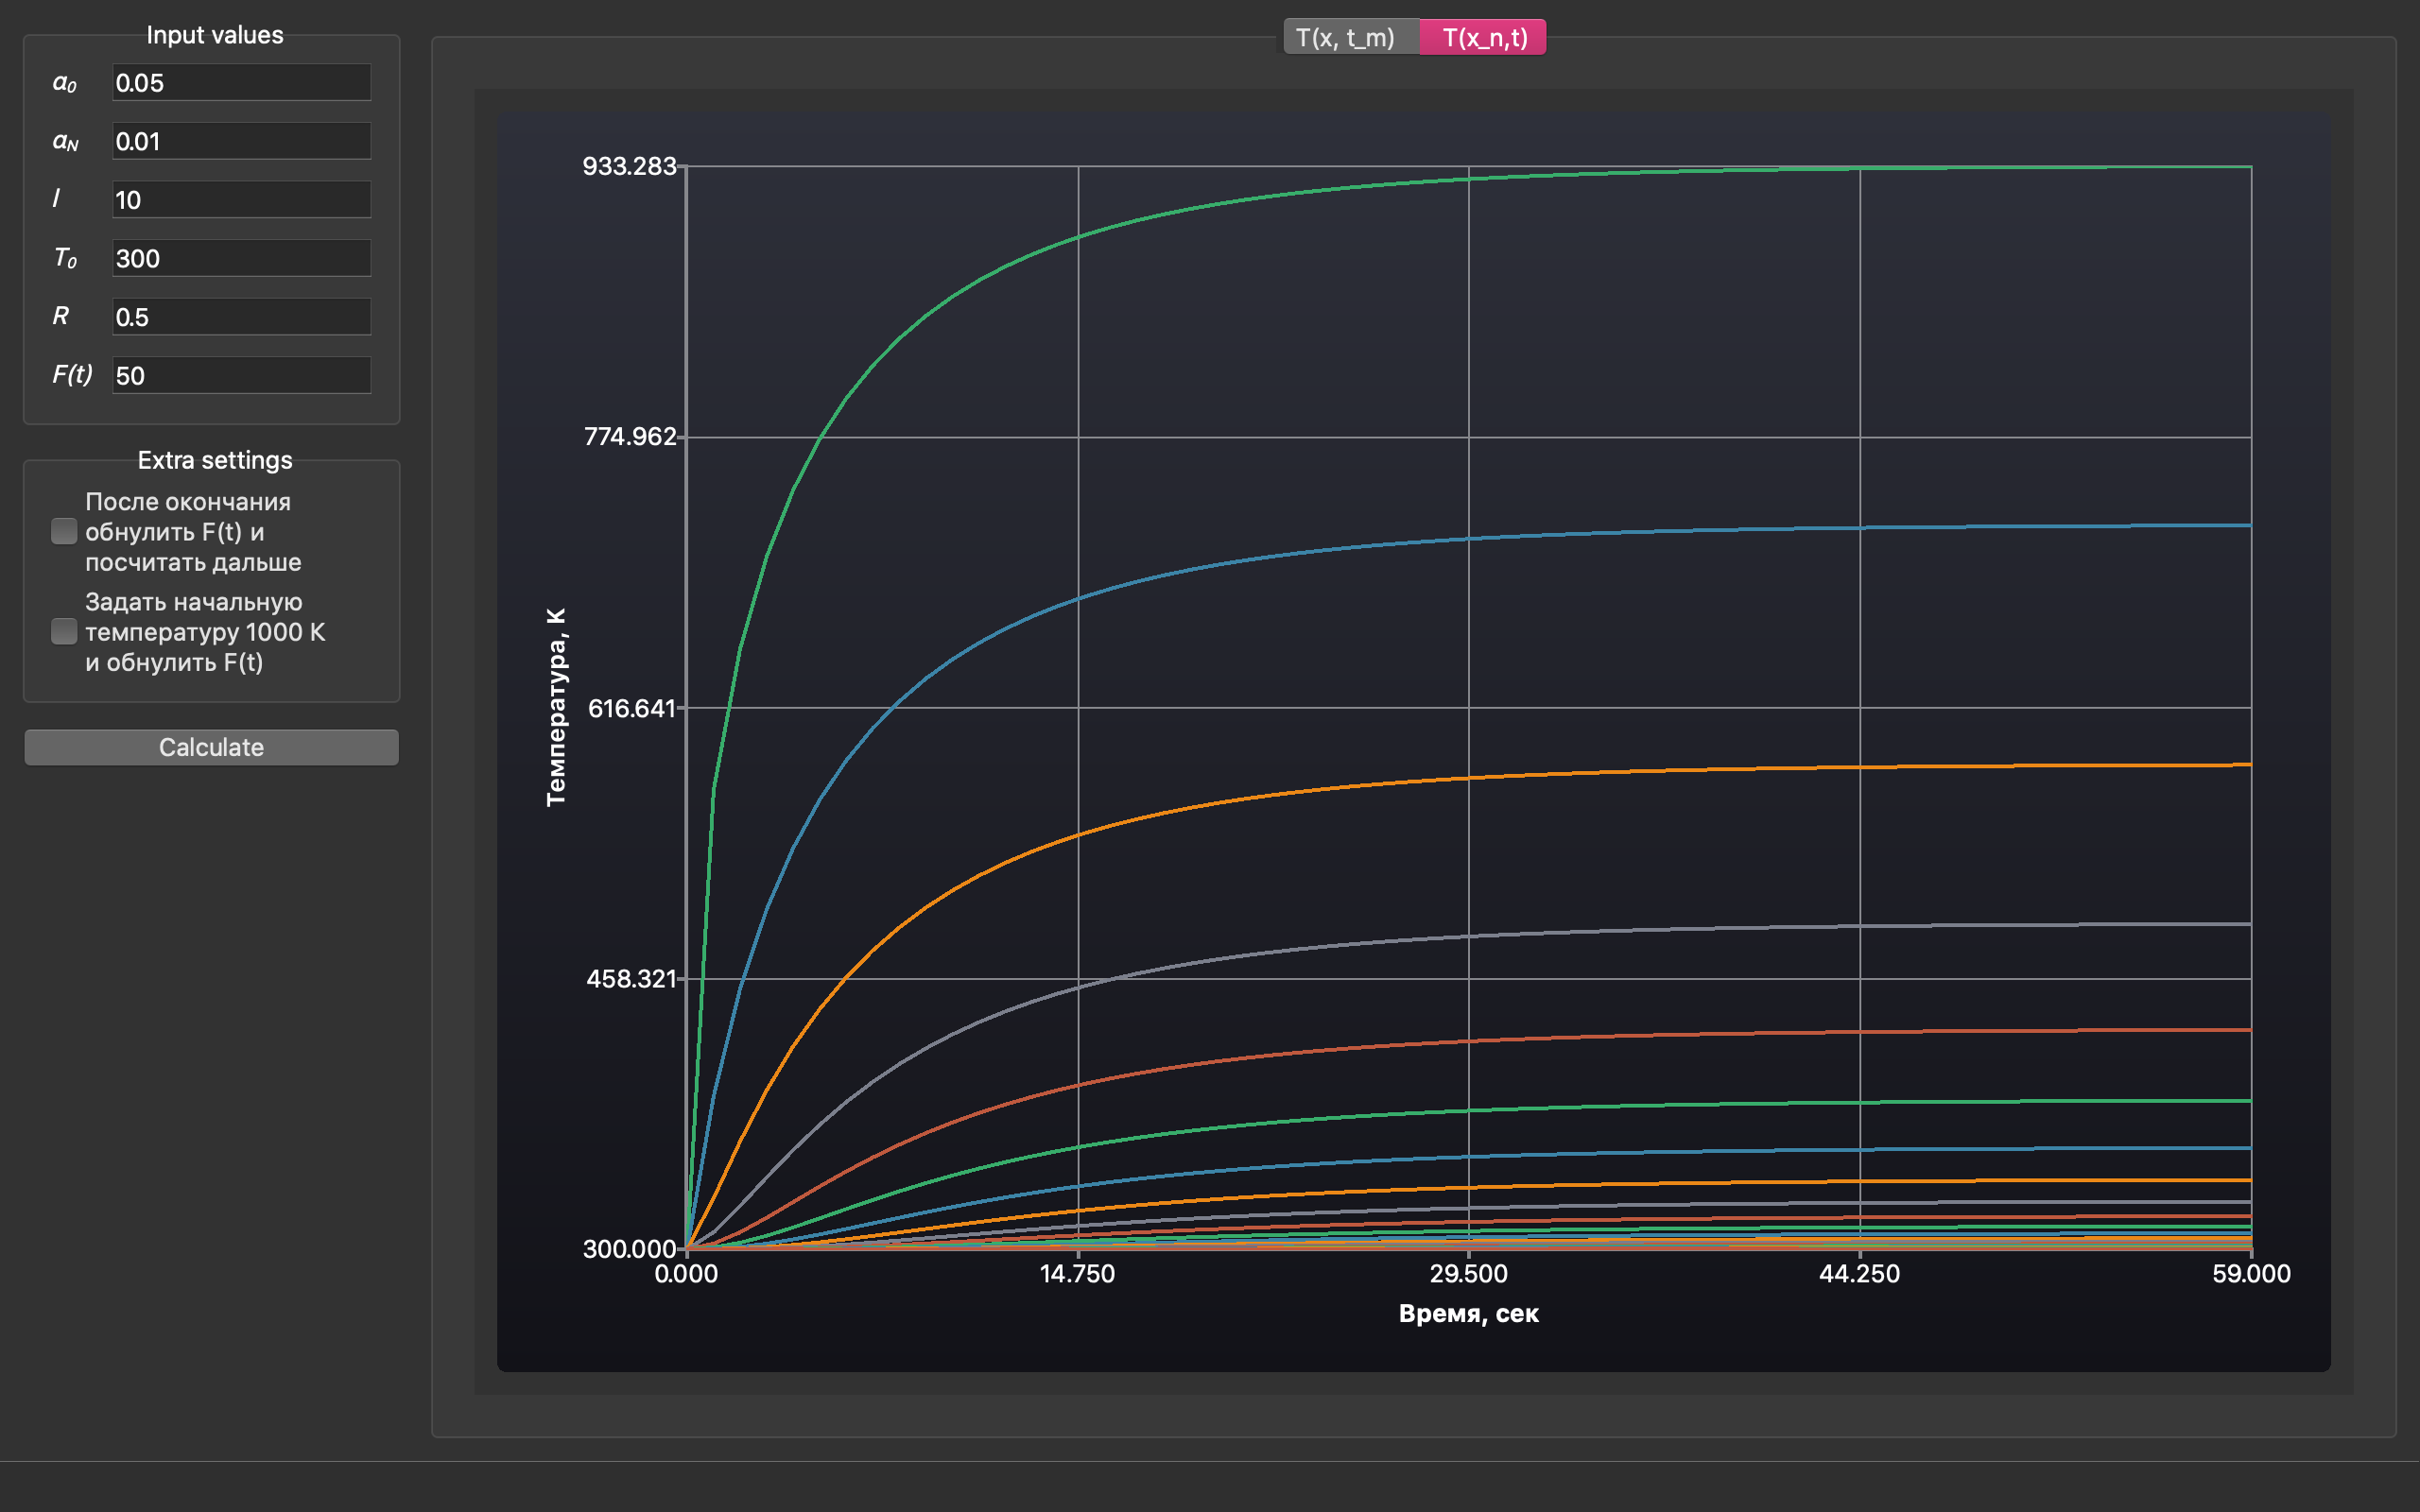
\includegraphics[scale=0.35]{img/defaultXn.png}
    \caption{Зависимость температуры от времени}
    \label{img:defaultXn}
\end{figure}

\section{ОТВЕТЫ НА ВОПРОСЫ}

\begin{enumerate}
    \item \textbf{Приведите результаты тестирования программы (графики, общие соображения, качественный анализ). Учесть опыт выполнения лабораторной работы №3.}

        На рисунке \ref{img:again} виден график (зависимость температуры от времени при фиксированных координатах стержня) в случае, когда после нагрева стержня мы устанавливаем поток равный 0 и запускаем вычисления заново с учетом последней температуры. В таком случае стержень после нагрева начнет остывать до температуры окружающей среды, которая равна 300 K.

        \begin{figure}[H]
            \centering
            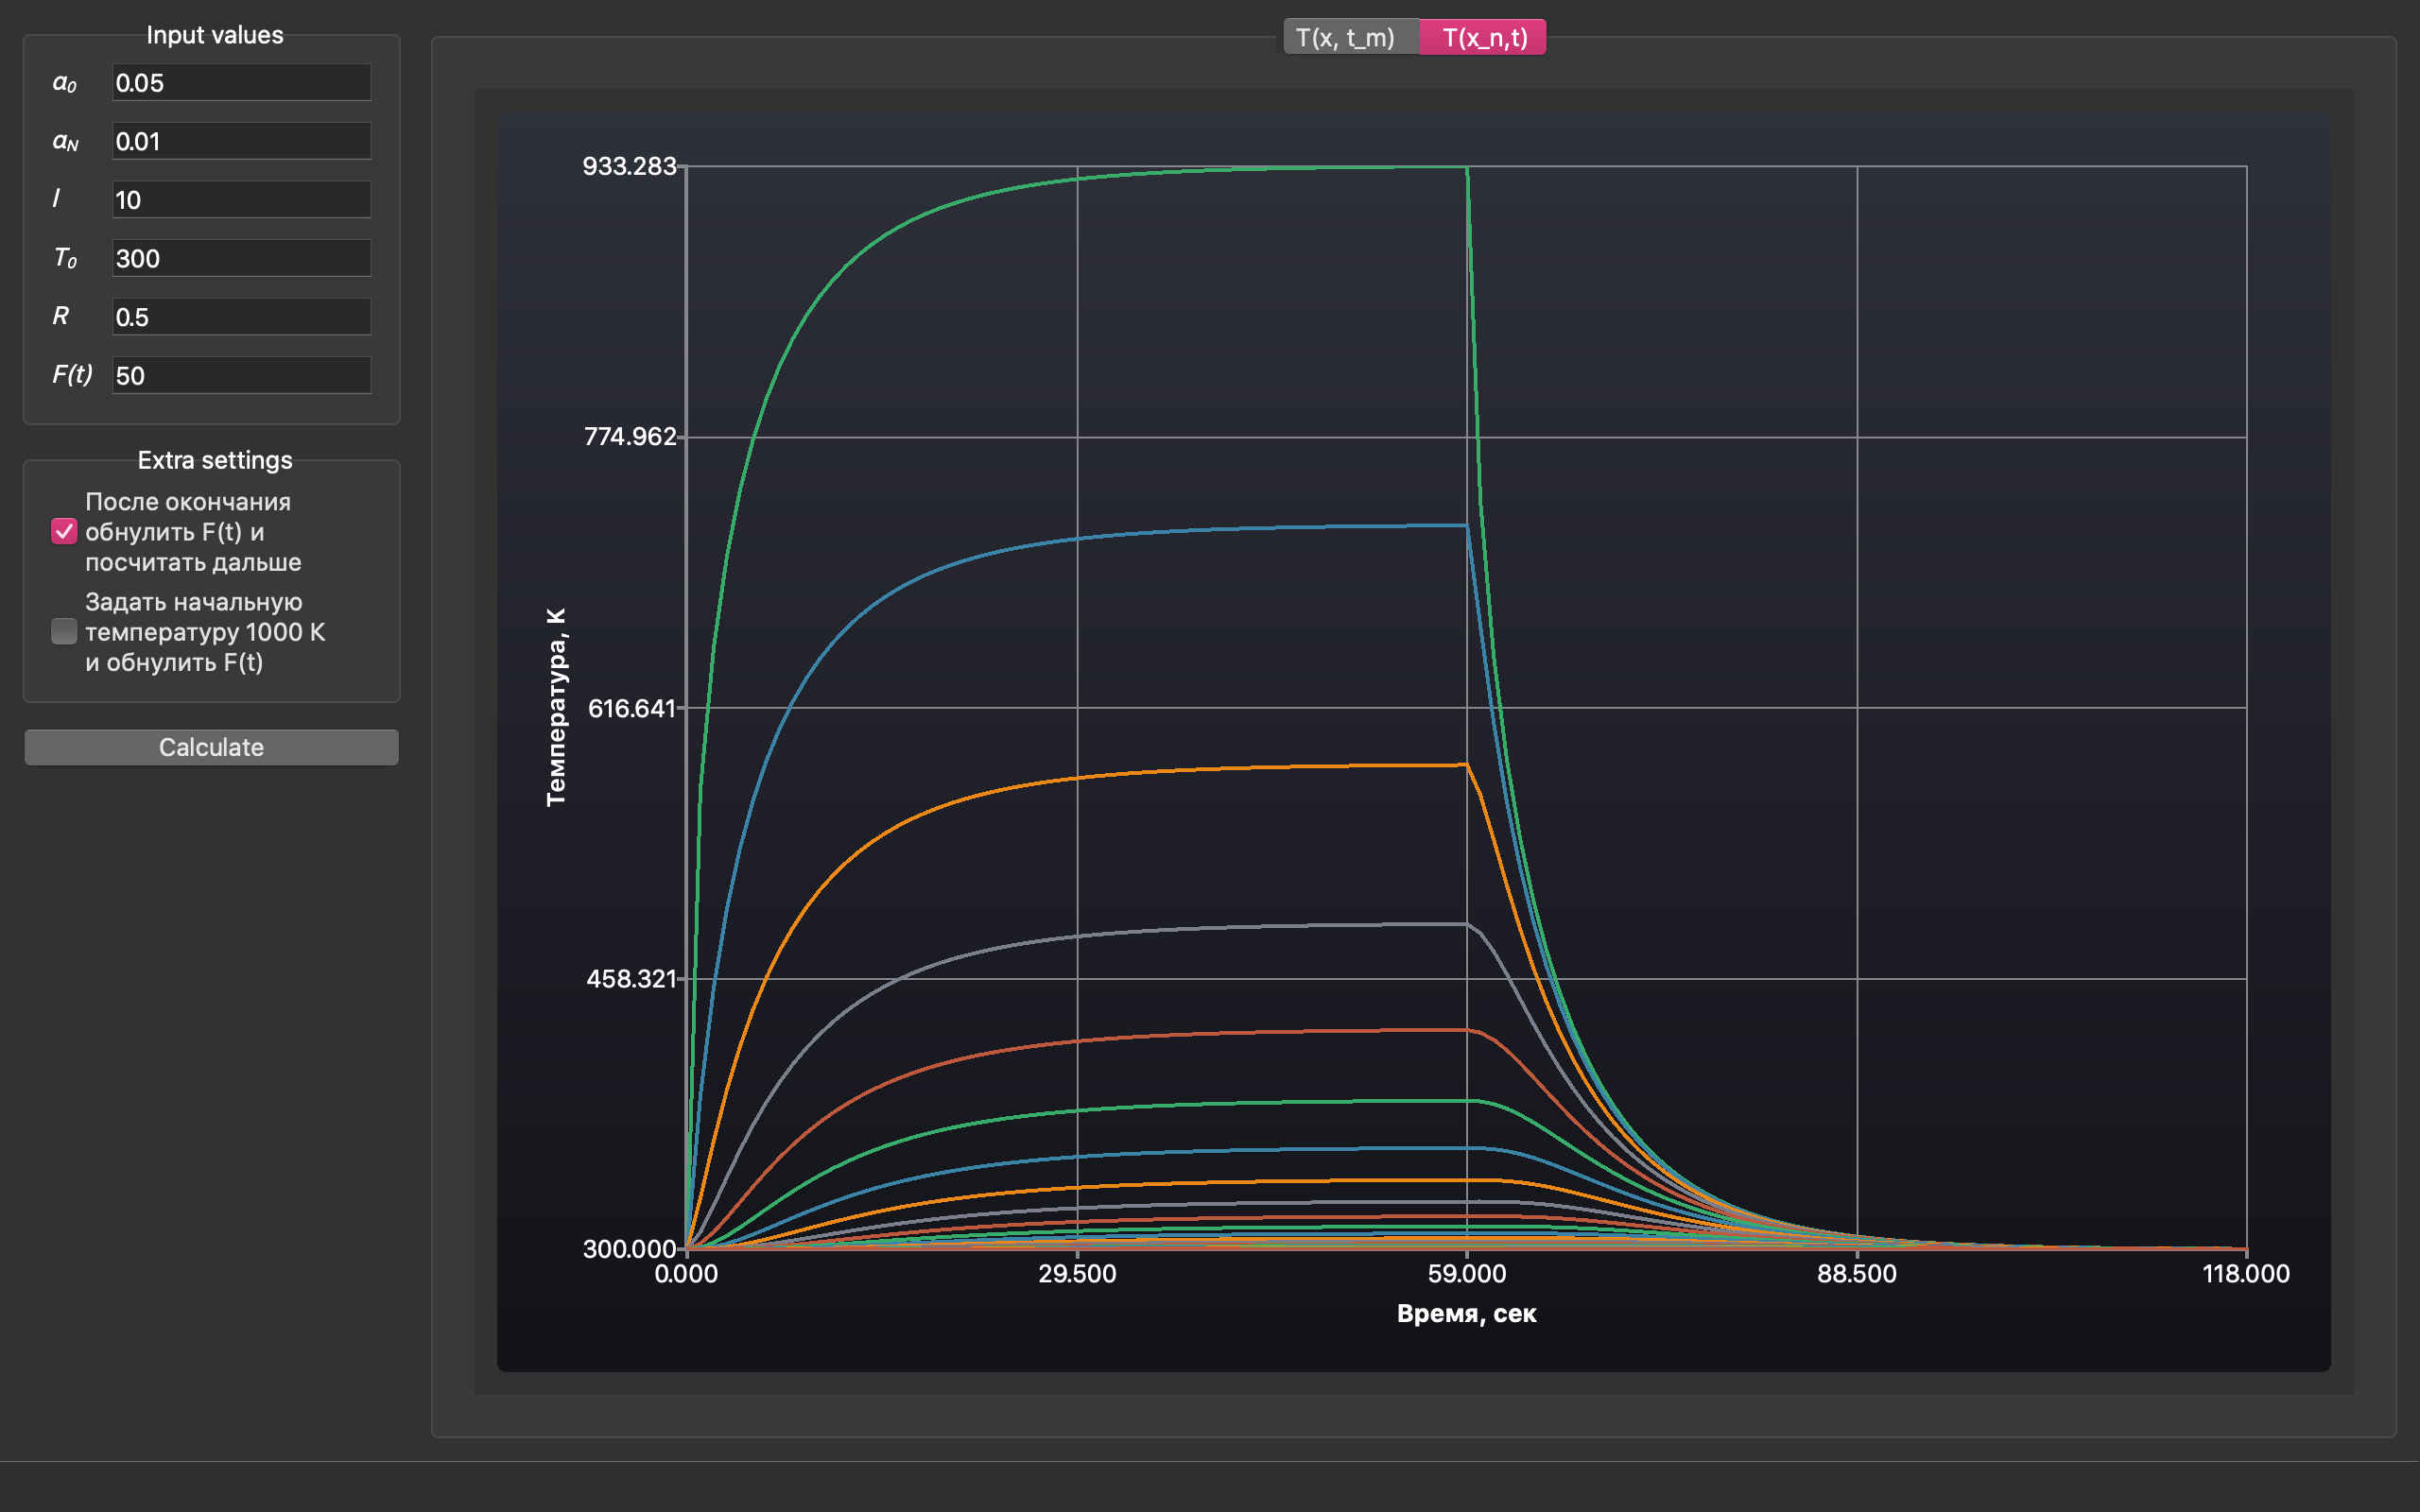
\includegraphics[scale=0.35]{img/again.png}
            \caption{Сначала нагрев стержня, затем остывание}
            \label{img:again}
        \end{figure}

        На рисунке \ref{img:start_temp} виден график (зависимость температуры от времени при фиксированных координатах стержня) в случае, если нагреть стержень до температуры 1000 К, а поток установить равным 0. В такой ситуации стержень будет остывать до тех пор, пока температура не станет равной температуре окружающей среды, которая равна 300 К.

        \begin{figure}[H]
            \centering
            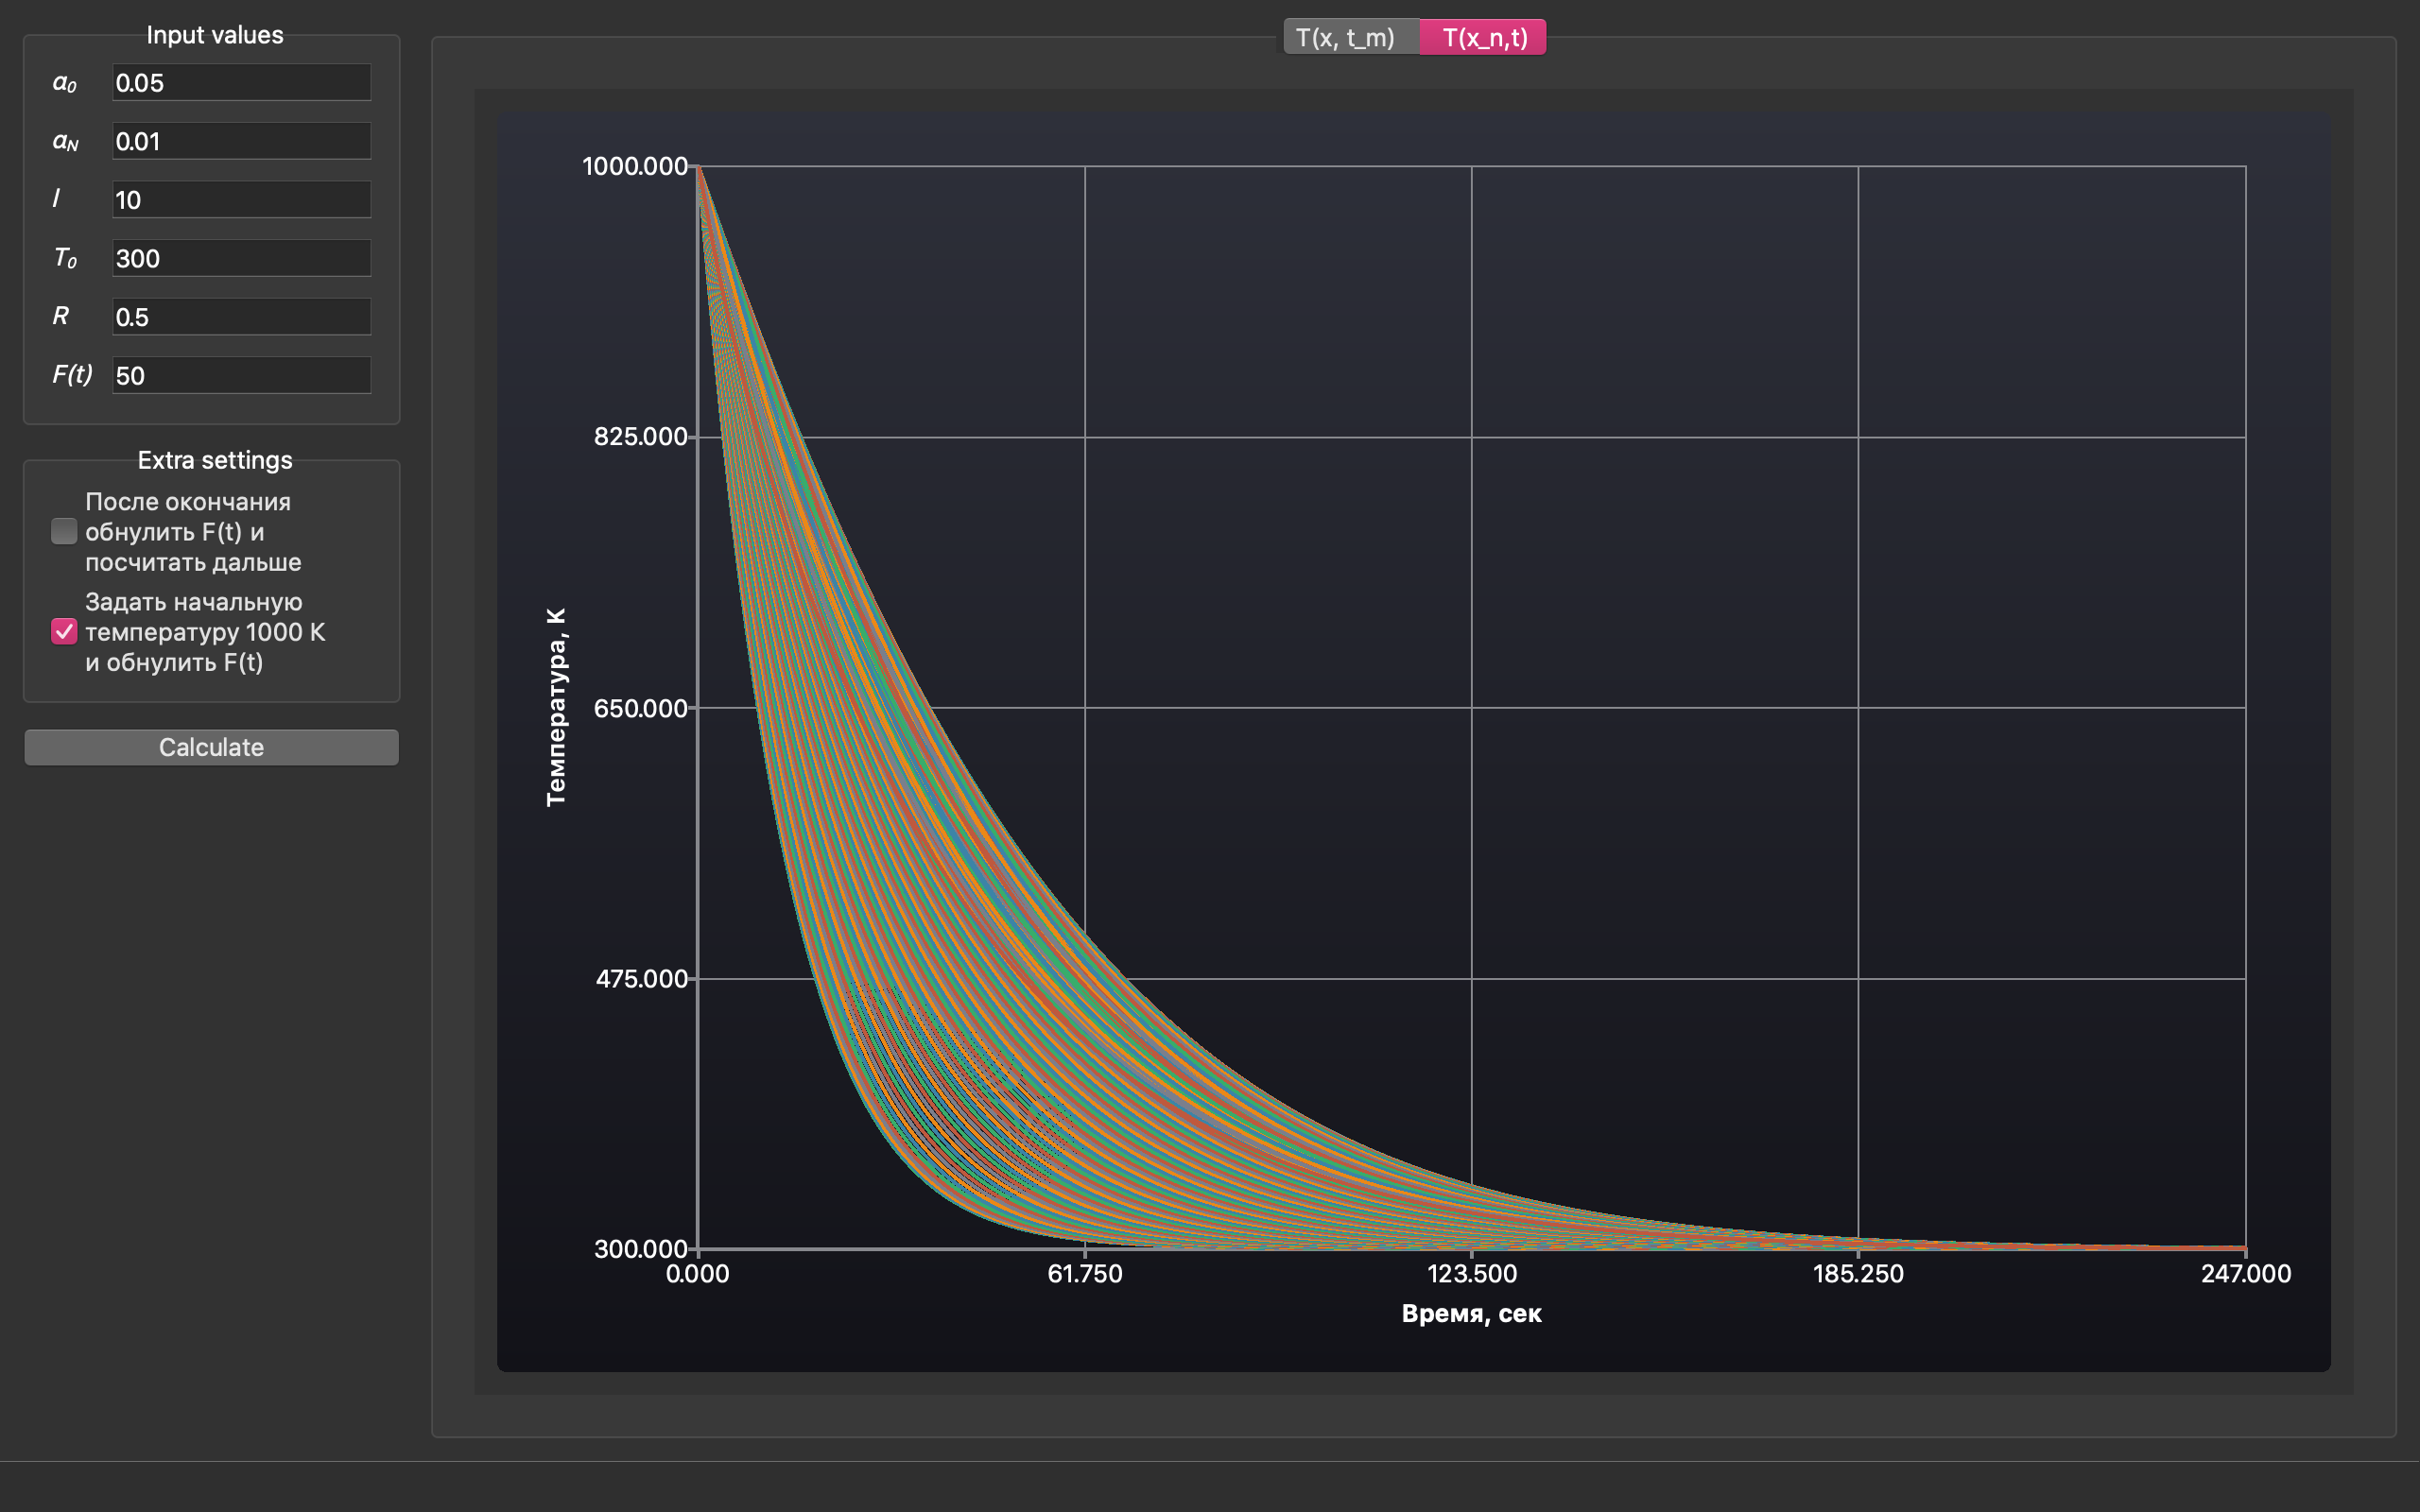
\includegraphics[scale=0.35]{img/start_temp.png}
            \caption{Стержень остывает до температуры 300 К}
            \label{img:start_temp}
        \end{figure}

        Если для коэффициента теплопроводности стержня поменять зависимость от $T$ на зависимость от $x$ как в третьей лабораторной, а теплоемкость стержня задать равной нулю, то график $T(x, t)$ из этой лабораторной работы (рисунок \ref{img:lab_03_new}) будет совпадать с графиком $T(x)$ из прошлой лабораторной работы (рисунок \ref{img:lab_03}).

        \begin{figure}[H]
            \centering
            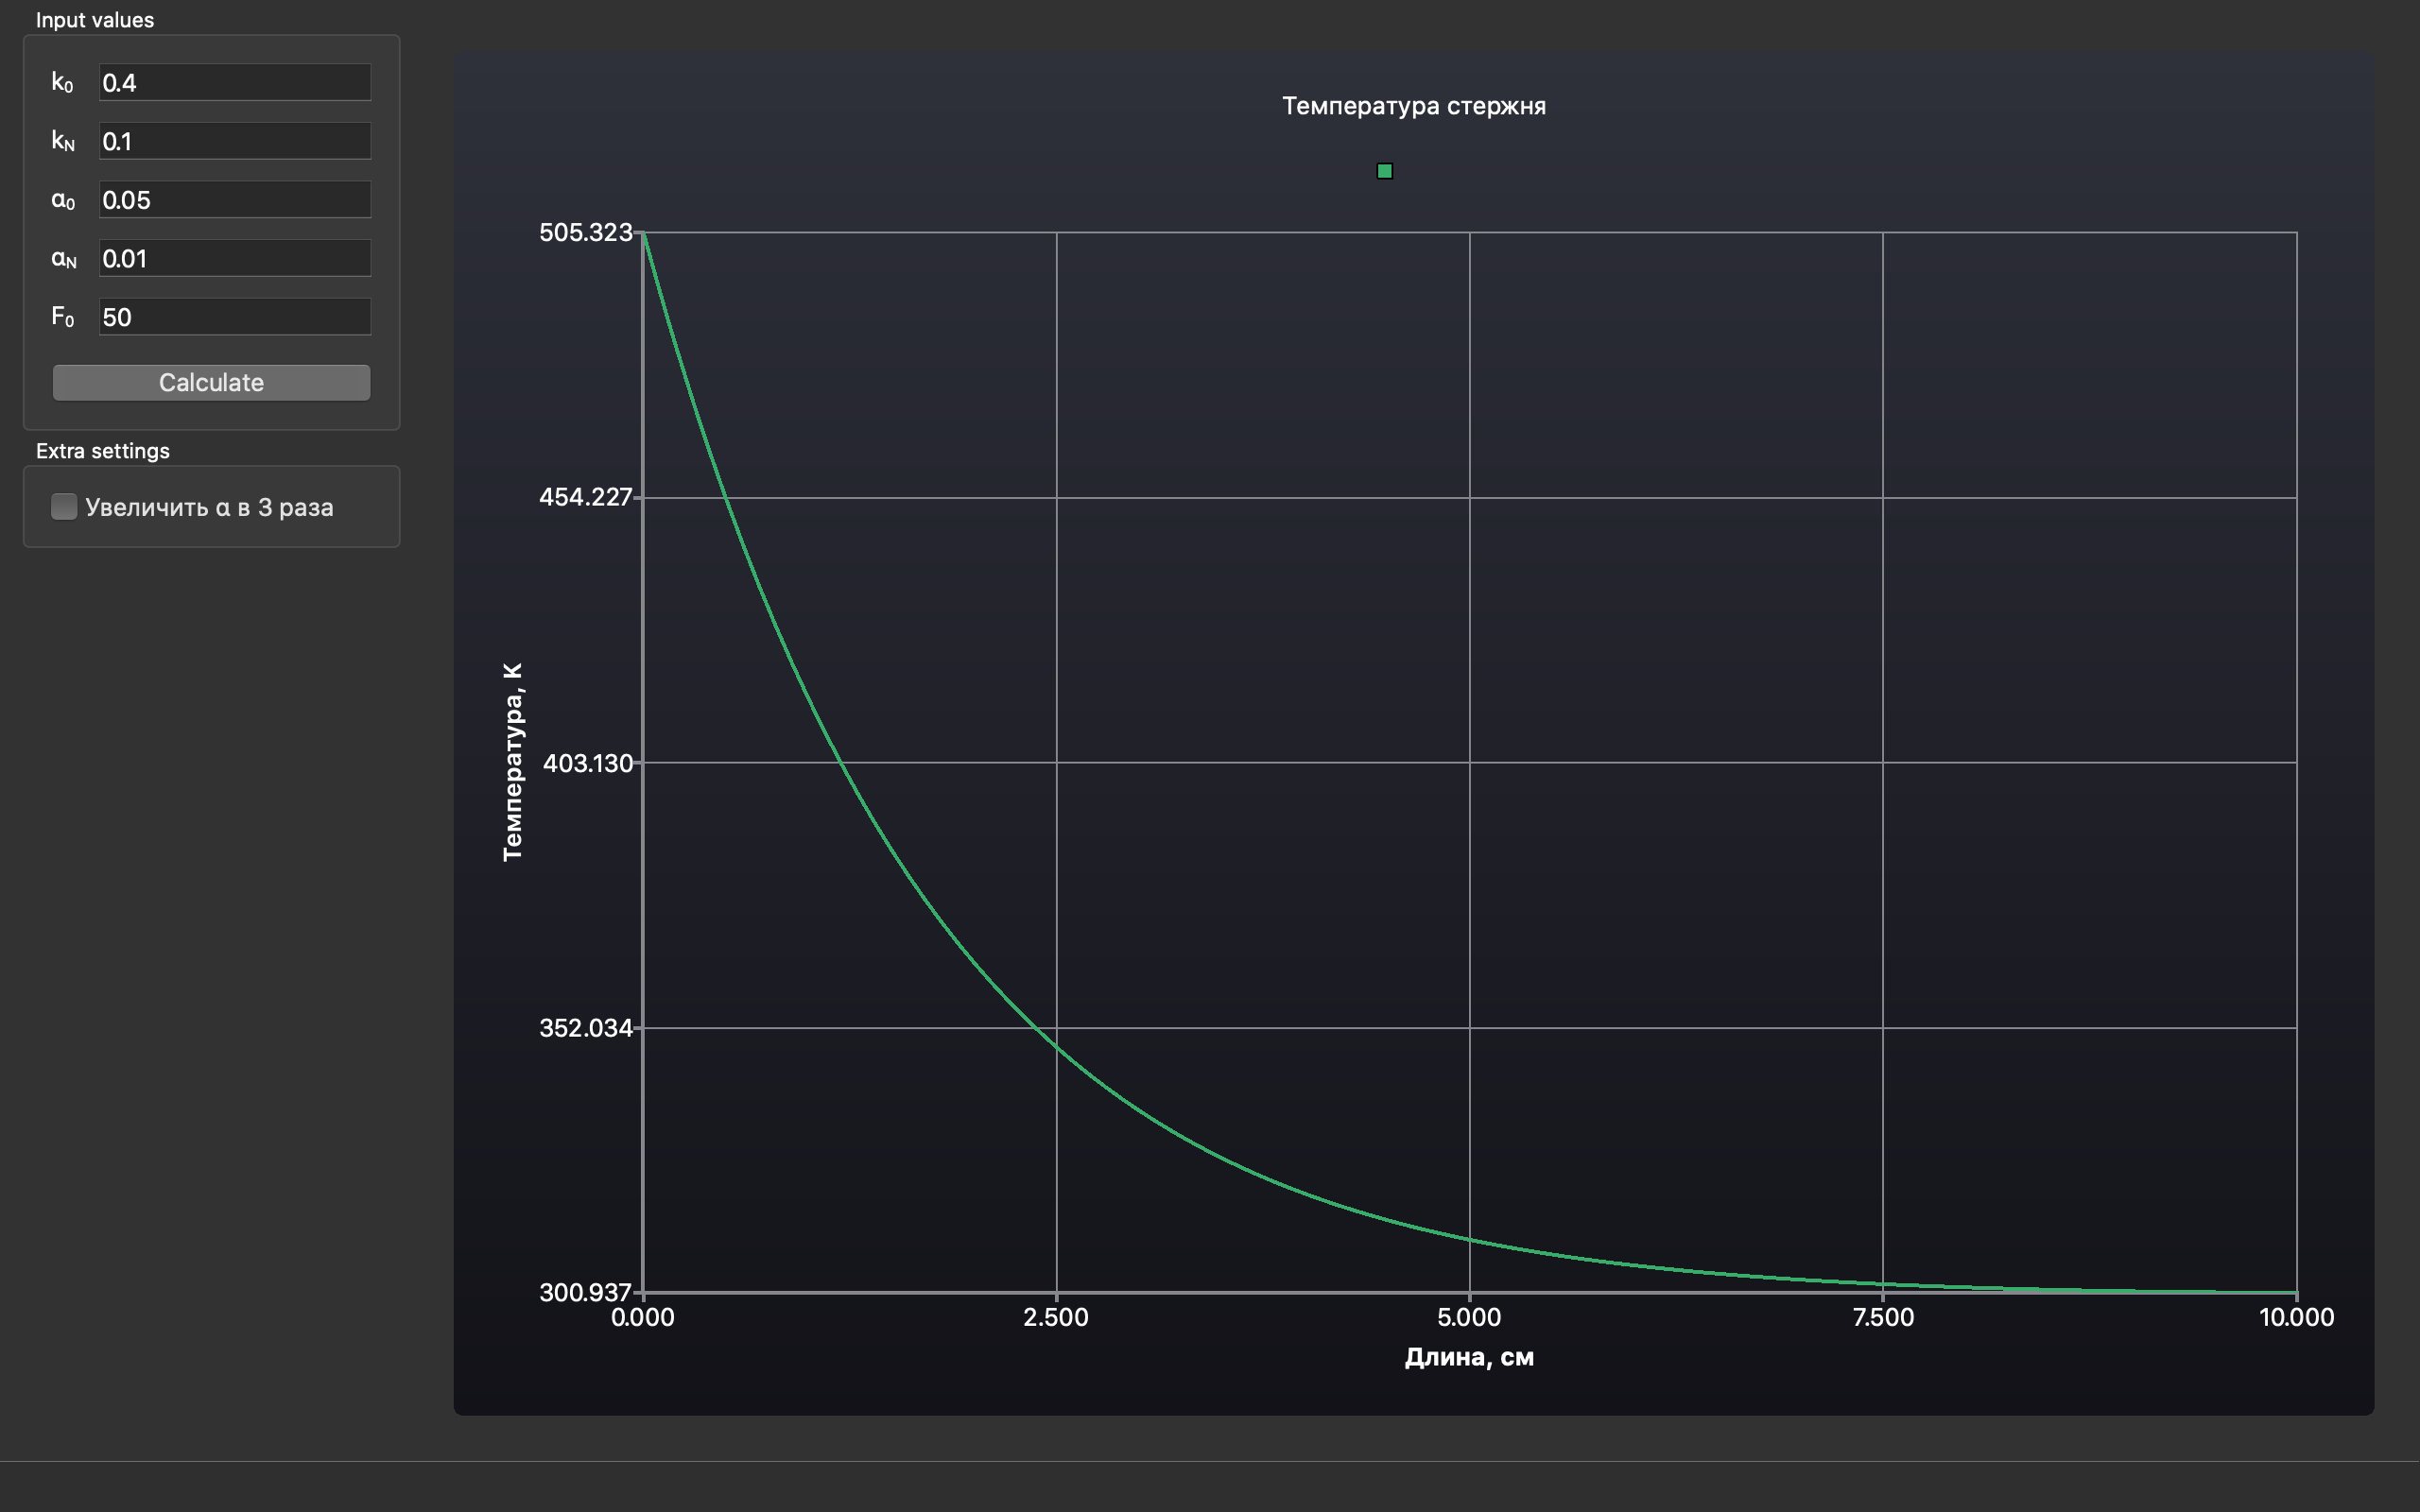
\includegraphics[scale=0.35]{img/lab_03.png}
            \caption{График из третьей лабораторной работы}
            \label{img:lab_03}
        \end{figure}

        \begin{figure}[H]
            \centering
            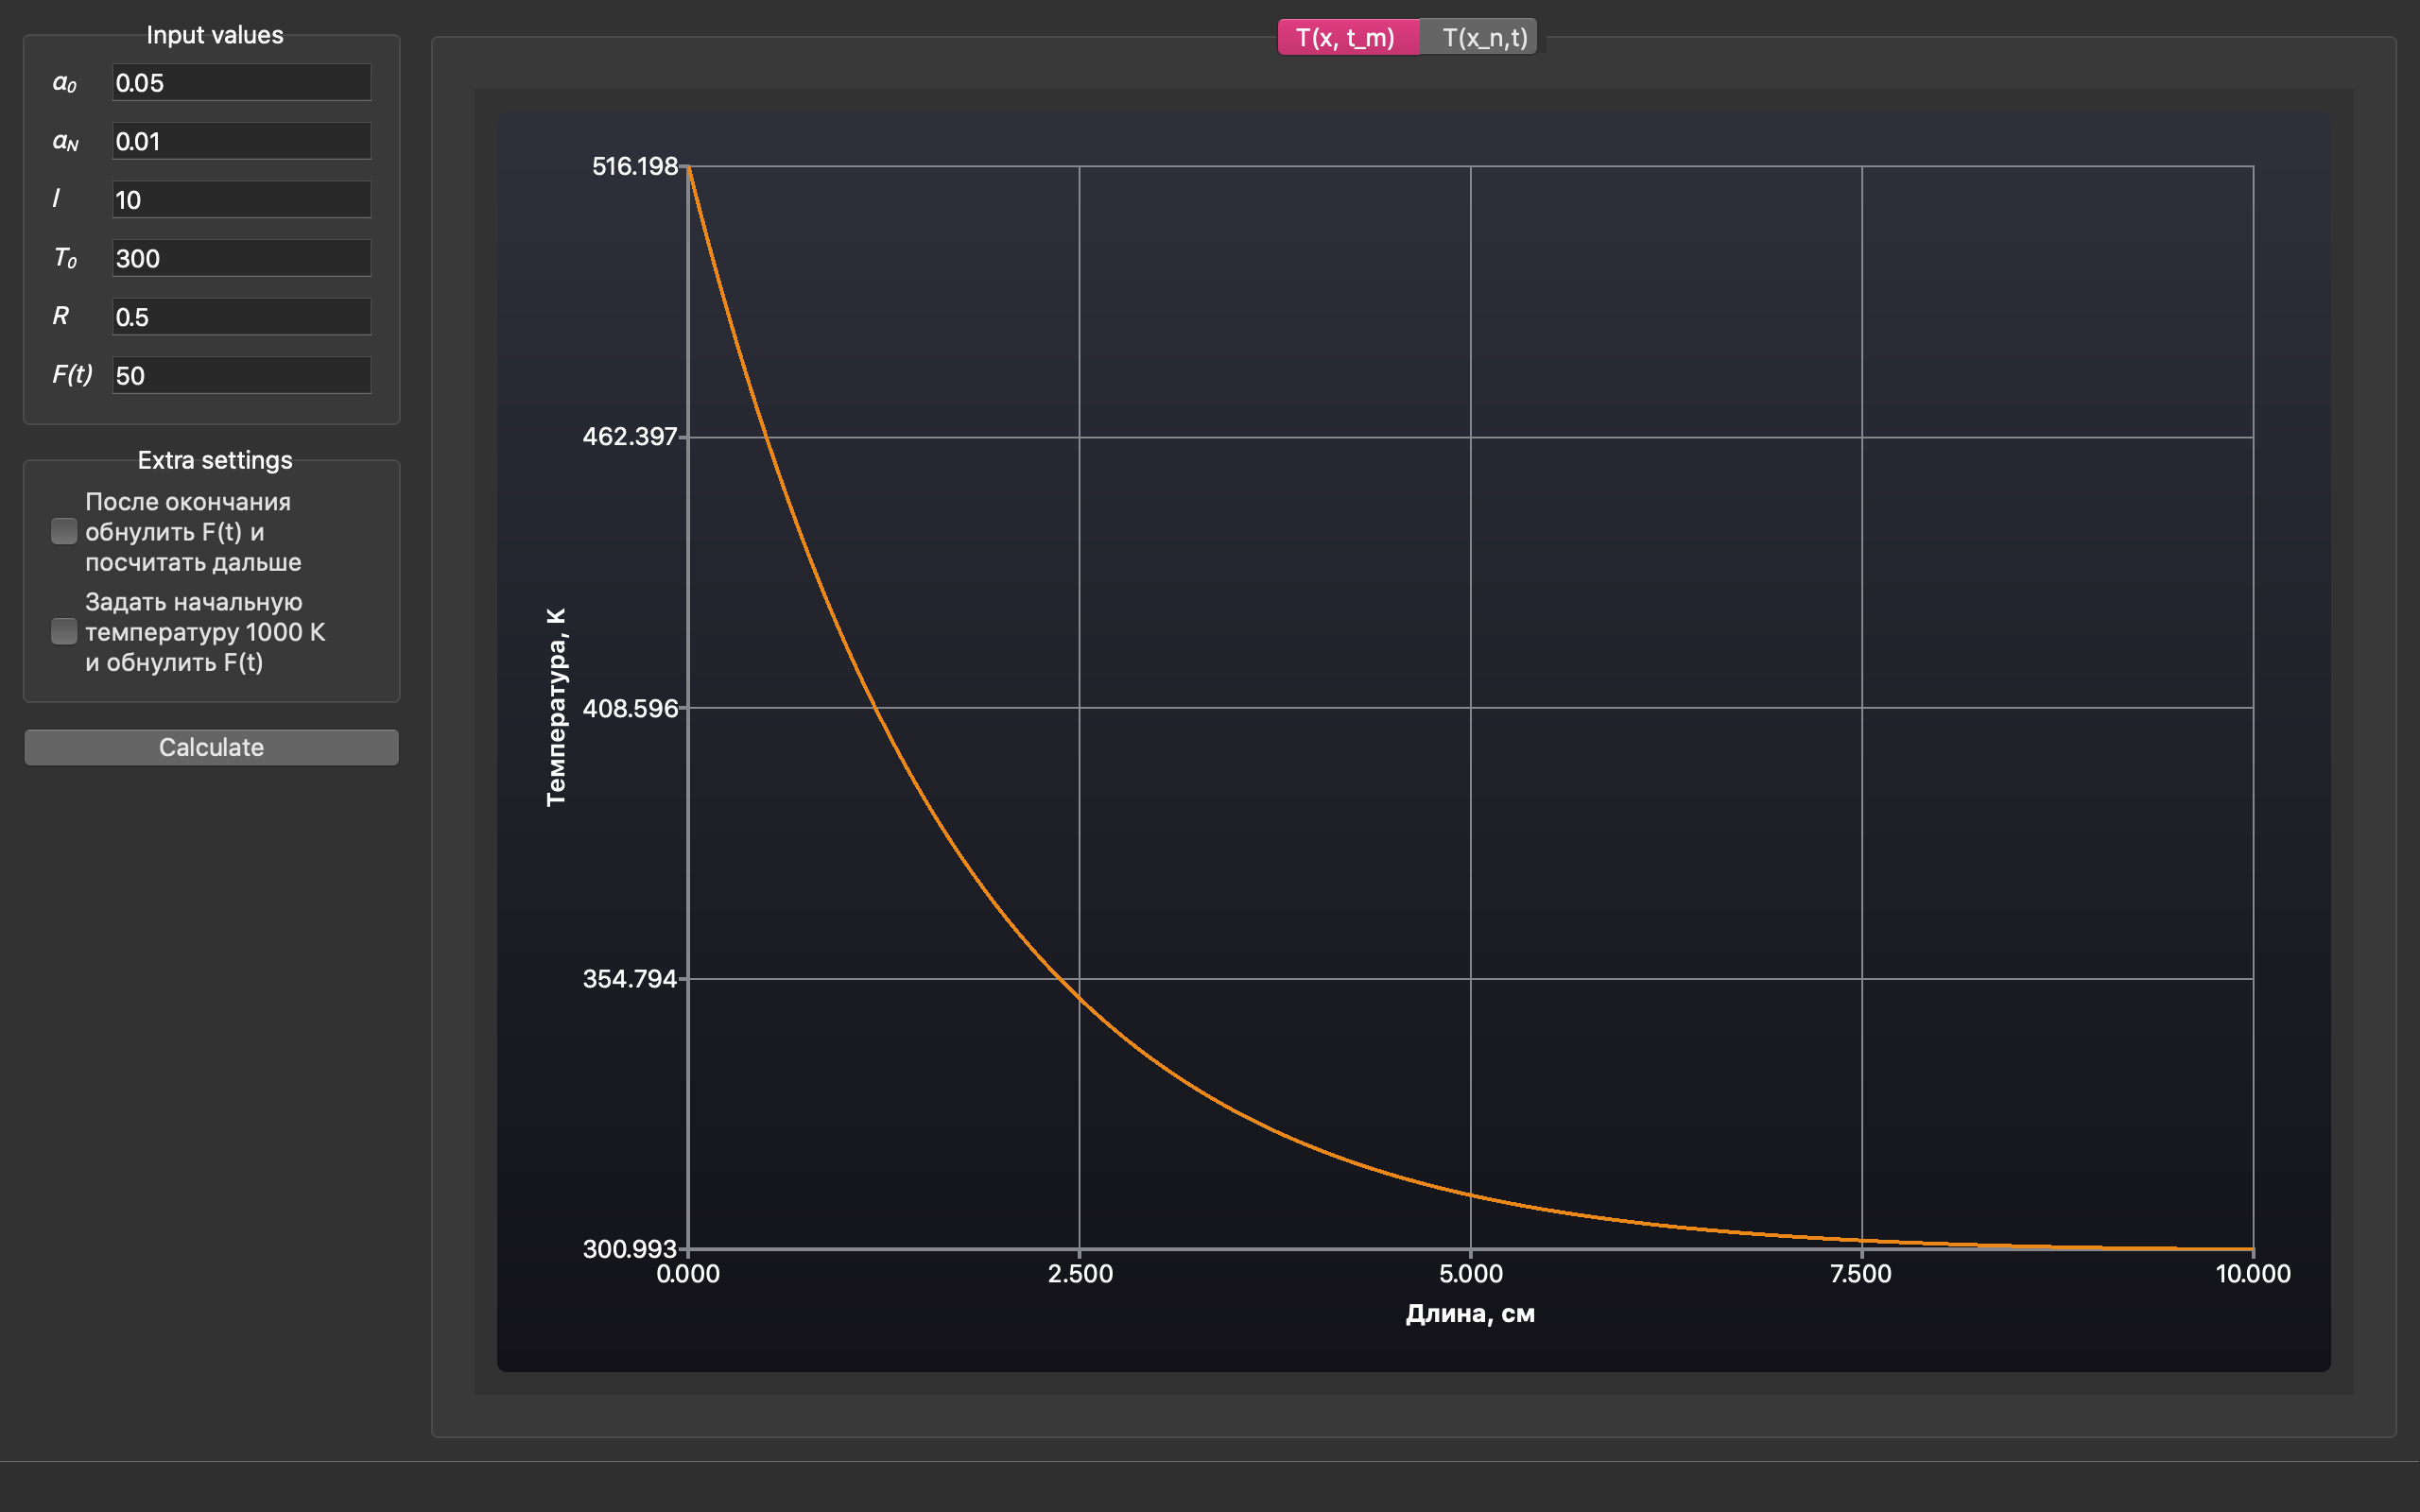
\includegraphics[scale=0.35]{img/lab_03_new.png}
            \caption{График из данной лабораторной работы}
            \label{img:lab_03_new}
        \end{figure}

    \item \textbf{Выполните линеаризацию системы \ref{eq:system_diff} по Ньютону, полагая для простоты, что все коэффициенты зависят только от одной переменной $y_n$. Приведите линеаризованный вариант уравнения и опишите алгоритм его решения.}

    \begin{equation*}
        \LittleCap{A}_n \LittleCap{y}_{n-1} - \LittleCap{B}_n \LittleCap{y}_n + \LittleCap{D}_n \LittleCap{y}_{n+1} = -\LittleCap{F}_n
    \end{equation*}

    Все коэффициенты зависят только от одной переменной, тогда

    \begin{multline*}
        \bigg( \LittleCap{A}_n \LittleCap{y}_{n-1} - \LittleCap{B}_n \LittleCap{y}_n + \LittleCap{D}_n \LittleCap{y}_{n+1} + \LittleCap{F}_n \bigg) \bigg|_{s-1} + \LittleCap{A}_n^{s-1} \Delta \LittleCap{y}_{n-1}^{s} + \\
        + \bigg( \frac{\partial \LittleCap{A}_n}{\partial \LittleCap{y}_n} \LittleCap{y}_{n-1} - \frac{\partial \LittleCap{B}_n}{\partial \LittleCap{y}_n} \LittleCap{y}_n - \LittleCap{B}_n + \frac{\partial \LittleCap{D}_n}{\partial \LittleCap{y}_n} \LittleCap{y}_{n+1} + \frac{\partial \LittleCap{F}_n}{\partial \LittleCap{y}_n} \bigg) \bigg|_{s-1} \Delta \LittleCap{y}_{n}^s + \\
        + \LittleCap{D}_n^{s-1} \Delta \LittleCap{y}_{n+1}^s = 0
    \end{multline*}

    Каноничный вид

    \begin{equation*}
        A_n \Delta \LittleCap{y}_{n-1}^s - B_n \Delta\LittleCap{y}_n^s + D_n \Delta \LittleCap{y}_{n+1}^s = -F_n
    \end{equation*}

    Тогда получаем, что

    \begin{equation*}
        \begin{matrix*}[l]
            A_n = \LittleCap{A}_n^{s-1} \\
            B_n = \bigg( -\frac{\partial \LittleCap{A}_n}{\partial \LittleCap{y}_n} \LittleCap{y}_{n-1} + \frac{\partial \LittleCap{B}_n}{\partial \LittleCap{y}_n} \LittleCap{y}_n + \LittleCap{B}_n - \frac{\LittleCap{D}_n}{\partial \LittleCap{y}_n} \LittleCap{y}_{n+1} - \frac{\LittleCap{F}_n}{\partial \LittleCap{y}_n} \bigg) \bigg|_{s-1} \\
            D_n = \LittleCap{D}_n^{s-1} \\
            F_n = \bigg( \LittleCap{A}_n \LittleCap{y}_{n-1} - \LittleCap{B}_n \LittleCap{y}_n + \LittleCap{D}_n \LittleCap{y}_{n+1} + \LittleCap{F}_n \bigg) \bigg|_{s-1} \\
        \end{matrix*}
    \end{equation*}

    Краевое условие для $y_0$

    \begin{equation*}
        \LittleCap{K}_0 \LittleCap{y}_0 + \LittleCap{M}_0 \LittleCap{y}_1 = \LittleCap{P}_0
    \end{equation*}

    Тогда

    \begin{equation*}
        \bigg( \LittleCap{K}_0 \LittleCap{y}_0 + \LittleCap{M}_0 \LittleCap{y}_1 - \LittleCap{P}_0 \bigg) \bigg|_{s-1} + \LittleCap{K}_0^{s-1} \Delta \LittleCap{y}_0^s + \LittleCap{M}_0^{s-1}\Delta \LittleCap{y}_1^s = 0
    \end{equation*}

    Каноничный вид

    \begin{equation*}
        K_0 \Delta \LittleCap{y}_0^s + M_0 \Delta \LittleCap{y}_1^s = P_0
    \end{equation*}

    Тогда получаем, что

    \begin{equation*}
        \begin{matrix*}[l]
            K_0 = \LittleCap{K}_0^{s-1} \\
            M_0 = \LittleCap{M}_0^{s-1} \\
            P_0 = \bigg( - \LittleCap{K}_0 \LittleCap{y}_0 - \LittleCap{M}_0 \LittleCap{y}_1 + \LittleCap{P}_0 \bigg) \bigg|_{s-1} \\
        \end{matrix*}
    \end{equation*}

    Краевое условие для $y_N$

    \begin{equation*}
        \LittleCap{K}_N \LittleCap{y}_N + \LittleCap{M}_{N-1} \LittleCap{y}_{N-1} = \LittleCap{P}_N
    \end{equation*}

    Тогда

    \begin{equation*}
        \bigg( \LittleCap{K}_N \LittleCap{y}_N + \LittleCap{M}_{N-1} \LittleCap{y}_{N-1} - \LittleCap{P}_N \bigg) \bigg|_{s-1} + \LittleCap{K}_N^{s-1} \Delta \LittleCap{y}_N^s+ \LittleCap{M}_{N-1}^s \Delta \LittleCap{y}_{N-1}^s = 0
    \end{equation*}

    Каноничный вид

    \begin{equation*}
        K_N \Delta \LittleCap{y}_N^s + M_{N-1} \Delta \LittleCap{y}_{N-1}^s = P_N
    \end{equation*}

    Тогда получается, что

    \begin{equation*}
        \begin{matrix*}[l]
            K_N = \LittleCap{K}_N^{s-1} \\
            M_{N-1} = \LittleCap{M}_{N-1}^s \\
            P_N = \bigg( -\LittleCap{K}_N \LittleCap{y}_N - \LittleCap{M}_{N-1} \LittleCap{y}_{N-1} + \LittleCap{P}_N \bigg) \bigg|_{s-1}\\
        \end{matrix*}
    \end{equation*}

    Система

    \begin{equation*}
        \begin{cases}
            K_0 \Delta \LittleCap{y}_0^s + M_0 \Delta \LittleCap{y}_1^s = P_0 \\
            A_n \Delta \LittleCap{y}_{n-1}^s - B_n \Delta\LittleCap{y}_n^s + D_n \Delta \LittleCap{y}_{n+1}^s = -F_n \\
            K_N \Delta \LittleCap{y}_N^s + M_{N-1} \Delta \LittleCap{y}_{N-1}^s = P_N \\
        \end{cases}
    \end{equation*}

    Решается методом прогонки, в результате находятся все $\Delta \LittleCap{y}_n^s$, после чего определяются значения искомой функции в узлах $\LittleCap{y}_n^s = \LittleCap{y}_n^{s-1} + \Delta \LittleCap{y}_n^s$. Итерационный процесс заканчивается при выполнении условия $\max \bigg| \frac{\Delta \LittleCap{y}_n^s}{\LittleCap{y}_n^s} \bigg| \le \varepsilon$.

\end{enumerate}
